\documentclass[12pt,a4paper]{article}
\usepackage[utf8]{inputenc}
\usepackage[german]{babel}
\usepackage{amsmath}
\usepackage{amsfonts}
\usepackage{amssymb}
\usepackage{graphicx}
\usepackage[numbers,round]{natbib}
\usepackage{url}
\author{}
\title{ Szenario-Prozess\\ Dokumentationsprotokoll\\ \textbf{Lehrerausbildung 2030} }
\begin{document}
\begin{titlepage}

\normalsize

\begin{flushleft}
Fachbereich Erziehungswissenschaft und Psychogie \\
Master - Studiengang Bildungswissenschaft \\
Wintersemester 2012/2013 \\
\end{flushleft}

\vspace{120pt}

\begin{center}
\huge
Szenario-Prozess\\ Dokumentationsprotokoll\\ \textbf{Lehrerausbildung 2030}
\vspace{60pt}
                         
\normalsize                               
Vorgelegt von Iryna Karpyuk\\
Matrikelnummer: 4222981
\end{center}                  
           
\begin{flushleft}
\normalsize
\vspace{100pt}

Seminar: Entwicklung in Bildungssystem und Bildungsforschung\\ 
Dozent: Sascha Danneberg\\
\vspace{60pt}

Berlin, 30.03. 2013
\end{flushleft}
\end{titlepage}
\normalsize                                              
\pagebreak

%Inhaltsverzeichnis
%Einleitung
%1.Theoretischer Hintergrund und Fragestellung
%2.Ziele des Szenarioprozesses und potenzielle Auftraggeber
%3.Abgrenzung des Themenfeldes
%4.Angabe des gewählten Zeithorizonts
%5.Beschreibung der wesentlichen Phasen und Arbeitsschritte des Szenario-Prozesses
\tableofcontents

\pagebreak

\section{Einleitung}

Die Zukunft ist ungewiss. Niemand kann mit Gewissheit vorhersagen, wie sie sich gestaltet. Es gibt immer mehrere gestaltbare und mögliche Zukünfte. Da die meisten Entscheidungen der Gegenwart in ihren Folgen zukunftbezogen sind, ist es jedoch notwendig, diese Folgen abschätzen und bewerten zu können. Mit diesem Anspruch untersucht die wissenschaftliche Zukunftsforschung gegenwärtige Zukünfte. Dabei wird versucht, verschiedene Alternativen zu entwickeln und die Wege zu beschreiben, auf denen bestimmte Entwicklungen erreicht werden könnten. Die so generierten Zukunftsbilder sind in der Lage, Orientierungs- und Handlungswissen zu liefern. Zukunftsforschung kann in vielen Bereichen angewendet werden – sie ist inter-, trans- und multidisziplinär und auch in der Lage großräumige und globale Zusammenhänge zu betrachten. Dabei bedient sie sich verschiedenen Instrumenten und Methoden, von denen eine die Szenario-Methode ist.
In der vorliegenden Arbeit soll der komplette Prozess von der Themenfindung über alle einzelnen Schritte eines solchen Szenario-Prozesses an einem konkreten Beispiel protokolliert werden. Das Dokumentationsprotokoll beginnt mit einen Überblick über die theoretischen Grundlagen der Szenario-Methodik, in dem die generellen Phasen eines Szenario-Prozesses, d.h. die Szenariofeldbestimmung, die Identifikation der Schlüsselfaktoren, die Analyse der Schlüsselfaktoren, die Szenario-Generierung und der Szenario-Transfer aufgegriffen und kurz erläutert werden. Zudem wird   auf methodische Hinweise bezüglich der Prozessschritte eingegangen, beispielsweise wie die Einflussanalyse, die Deskriptorenanalyse sowie die Entwicklung von Szenarien, Strategien und Maßnahmen zur Problemlösung. Die theoretischen Grundlagen schließen mit den Kriterien für die Erstellung von Szenarien ab. Im zweiten Schritt geht es um den Forschungsgegenstand und die Forschungsfrage. Hier wurden wichtige Fragen zu den Adressaten, zu den Zielen, zum Nutzen und zum Betrachtungszeitraum beantwortet. Nach dem Abschluss des theoretischen Bereichs des Szenario-Prozess, folgt die eigentliche Dokumentation der einzelnen Phasen und Arbeitsschritte. Abschließend werden die wichtigsten Erkenntnisse zusammengefasst.

\section{Beschreibung der wesentlichen Phasen und Arbeitsschritte des Szenario-Prozesses}
Der typische explorative Szenario-Prozess lässt sich nach Kosow \& Gaßner (2008) \cite{Kosow2008} in fünf Phasen unterteilen: die Szenariofeldbestimmung, die Identifikation der Schlüsselfaktoren, die Analyse der Schlüsselfaktoren, die Szenario-Generierung und ggf. der Szenario-Transfer. Wobei der Szenario-Prozess im engeren Sinne nur aus den ersten vier besteht, da die letzte Phase optional gesehen wird und in diesem Projekt keine Umsetzung stattfindet. Die zentrale Bedeutung für alle Phasen ist, dass Auswahlschritte vorgenommen und begründet werden (vgl. Kosow/Gaßner 2008, S. 19-20).

\subsection{Szenariofeldbestimmung }
Szenario-Prozess beginnt mit der Szenariofeldbestimmung. Ziel der ersten Phase ist es, den Forschungsgegenstand genau zu bestimmen und gegenüber anderen abzugrenzen. Hierfür wird das Problem definiert, sowie was alles zum Problemfeld gehört bzw. was nicht dazu gehört. Hierbei findet eine thematisch-inhaltliche Beschränkung der Themen statt, die mit einbezogen werden sollen (vgl. Kosow/Gaßner 2008, S. 20). 

\subsection{Identifikation der Schlüsselfaktoren} 
In der zweiten Phase wird das Szenariofeld durch Schlüsselfaktoren beschrieben. Wichtig für die Identifikation sind Kenntnisse über das Feld und Kenntnisse über die Zusammenhänge der einzelnen Schlüsselfaktoren (vgl. Kosow/Gaßner 2008, S. 21). „Schlüsselfaktoren (...) sind die zentralen Größen, die das Szenariofeld beschreiben bzw. die auf das Feld wirken und/ oder über die das Feld nach außen wirkt. Schlüsselfaktoren sind diejenigen Variablen, Parameter, Trends, Entwicklungen und Ereignisse, die im weiteren Verlauf des Szenario-Prozesses zentral betrachtet werden.“ (vgl. Kosow/Gaßner 2008, S. 21) 

\subsection{Analyse der Schlüsselfaktoren} 
Die Analyse der Schlüsselfaktoren nimmt laut Literatur ein sehr prägenden Einfluss auf die Szenariomethode. Die einzelnen Schlüsselfaktoren werden daraufhin analysiert, welche möglichen zukünftigen Ausprägungen jeweils vorstellbar sind. Ausgewählt werden jene Ausprägungen, die in die Szenario-Bildung einfließen sollen. In der Praxis kann dieser Schritt auf vielfältige Weise durchgeführt werden. Es wird in der Literatur stets erwähnt, dass die intuitiv-kreativen Aspekte von besonderer Notwenigkeit sind, um die zukünftigen Entwicklungen eines Schlüsselfaktors herauszuarbeiten und vorstellen zu können (vgl. Kosow/Gaßner 2008, S. 21). 

\subsection{Szenario-Generierung} 
Für die Generierung der Szenarien ist es zunächst notwendig die zuvor herausgearbeiteten Ausprägungen zu bündeln und zu verdichten. Diese herausgearbeiteten „Faktorenbündel“ werden zur konkreten Szenario-Bildung herangezogen. Methodisch gibt es auch hier unterschiedliche Herangehensweisen, es kann nach narrativ-literarischen bis hin zu formalisiert-mathematischen Verfahren erfolgen (vgl. Kosow/Gaßner 2008, S. 21). Anschließend gilt es aus der Vielzahl der möglichen Szenarien eine Auswahl von vier bis fünf zu treffen, um eine kognitive Überforderung der Adressaten zu vermeiden. 

\subsection{Szenario-Transfer (optional)} 
Diese Phase beschreibt die weitere Verwendung und/ oder Verarbeitung der erstellten Szenarien. Sie wird nur bei einigen Szenario-Techniken explizit zum Szenario-Prozess selbst gezählt. Wie in den meisten Phasen des Prozesses besteht auch hier eine große Umsetzungsvielfalt, für die weitere Verwendung der erstellten Szenarien. So besteht beispielsweise die Möglichkeit mit Wirkungsanalysen, Akteurs-Analysen, Strategiebewertung und -Entwicklung weitere Schritte zu tätigen. Der Fokus liegt darauf, die Unterschiede zwischen den verschiedenen Szenarien zu sehen und Merkmale zur Unterscheidung und Charakterisierung verschiedener Szenario-Ansätze hervorzuheben (vgl. Kosow/Gaßner 2008, S. 22). 

\section{Methodische Hinweise für die Prozessschritte}
Die Szenario-Methode gliedert sich in verschiedene Phasen. In der Literatur existieren dazu unterschiedliche Ausgestaltungen. Nach Albers und Broux (1999)\cite{Albers1999} gliedern sich die Phasen wie folgt: 

\subsection{Aufgaben- und Problemanalyse} 
In diesem Prozessschritt wird der Sachverhalt genau festgelegt und beschrieben. Die Auseinandersetzung mit der Gegenwart stellt die Basis der Szenarien dar, somit muss erst der Ist-Zustand beschrieben werden. Dementsprechend muss ein bestimmtes Grundwissen über das Thema vorhanden sein bzw. muss man sich durch Literatur ein Basiswissen aneignen. Ziel dieses Schrittes ist, dass am Ende der Auseinandersetzung mit dem Thema eine bestimmte Problematik bzw. Problembeschreibung sichtbar werden soll (vgl. Albers/Broux 1999, S. 61). 

\subsection{Einflussanalyse} 
In dieser Phase geht es zunächst darum, bestimmte Faktoren zu ermitteln, die den Untersuchungsgegenstand bzw. das gewählte Thema beschreiben und beeinflussen. Um diese Faktoren miteinander in Verbindung zu bringen, kann es nützlich sein, sie gegenüber zu stellen. Dies kann mithilfe einer Matrix dargestellt werden. Die Matrix dient der Übersicht, dabei kommt es nicht so sehr auf die Ergebnisse an, sondern veranschaulicht die Zusammenhänge der Faktoren (vgl. Albers/Broux 1999, S. 62 f). 

\subsection{Deskriptorenanalyse} 
In diesem Schritt werden die Einflussfaktoren bewertet. Dazu müssen die Faktoren als Deskriptoren beschrieben werden, d.h. sie müssen genauer beschrieben werden, sodass sie klar verständlich sowie qualitativ oder quantitativ und sachlich formuliert sind. Die Deskriptoren werden dann in ihrem künftigen Entwicklungsverlauf analysiert und bewertet (vgl. Albers/Broux 1999, S. 63). 

\subsection{Entwicklung der Szenarien} 
Hier werden ausführliche Szenarien aufgestellt. Mit Hilfe der Ergebnisse aus den vorangegangenen Phasen sollen anschauliche Zukunftsentwicklungen entstehen. Diese Entwicklung können unter anderem auch fiktiv sein, es ist aber wichtig die Konsequenzen der Szenarien sichtbar zu machen (vgl. Albers/Broux 1999, S. 64). 

\subsection{Entwicklung von Strategien und Maßnahmen zur Problemlösung} 
In der letzte Phase sollen Konsequenzen aus den Szenarien gezogen werden. Dies führt zu einer Problemanalyse der Ausgangssituation, denn es sollen Strategien entworfen werden, die einen positiven Verlauf der Ausgangssituation möglich machen (vgl. Albers/Broux 1999, S. 64). 

\section{Kriterien für die Erstellung von Szenarien} 
Nach Reibnitz (1992)\cite{Reibnitz1992} müssen Szenarien folgenden Kriterien entsprechen: 

1. Größtmögliche Stimmigkeit, Konsistenz und Widerspruchsfreiheit, d.h. die einzelnen Entwicklungen innerhalb eines Szenarios dürfen sich nicht gegenseitig aufheben. 
2. Größtmögliche Stabilität des Szenarios, d.h. die Szenarien dürfen nicht bei kleineren Erschütterungen oder Veränderungen einzelner Faktoren zusammenbrechen. 
3. Größtmögliche Unterschiedlichkeit der Grundtypen, d.h. man soll bei der Ausgestaltung der Extrem-Szenarien mög"-lichst nahe an die Ränder des Trichters herankommen.

Kosow \& Gaßner (2008) stellen dagegen folgende Kriterien zusammen: 
1. Plausibilität: die dargestellten Entwicklungen müssen möglich sein. 
2. Konsistenz: die Zukunftspfade und Bilder innerhalb eines Szenarios müssen in sich stimmig sein. 
3. Verständlichkeit: die dargestellten Entwicklungen und Zukunftsbilder müssen nachvollziehbar sein. 
4. Trennschärfe: ausgewählte alternative Szenarien müssen sich in genügend hohem Maße unterscheiden. 
5. Transparenz: deutliche Kennzeichnung und Begründung der zugrundeliegenden Annahmen/Werturteile und Auswahlentscheidungen sowie Rahmenbedingungen. 

\section{Theoretischer Hintergrund und Fragestellung} 

Die gesteigerte Aufmerksamkeit der Medien, eine Vielzahl neuerer wissenschaftlicher Publikationen sowie eine intensive bildungspolitische Debatte deuten auf die große Bedeutung des Themas „Lehrerbildung in Deutschland“. Dabei besteht in der Lehrerbildungsdiskussion überwiegend Einigkeit über die Mängel insbesondere der Lehrerausbildung, die sich in Deutschland in eine erste, universitäre und eine zweite, berufsfeldorientierte Phase untergliedert. Ebenso wie an Kritik mangelt es auch nicht an entsprechenden konzeptionellen und programmatischen Vorschlägen zur Verbesserung der Lehrerbildung (vgl. Schaefers 2002, S. 65)\cite{Christine2002}. Vor allem aber ist in der Realisierung der neuen Lehrerbildung eine Heterogenität der Programme nicht nur zwischen den Ländern, sondern selbst zwischen den einzelnen Hochschulen charakteristisch, neue Lehr- und Lernformen sind bisher nicht ausreichend entwickelt, die konkrete Umsetzung bleibt stehen, die Kooperation der unterschiedlichen Phasen ist eher Forderung als Realität

(vgl. Entschließung des 206. Plenums 2006, S. 7) \cite{Hochschulrektorenkonferenz2006}. 
 
Die Kritik an der Lehrerbildung hält in der allgemeinen Öffentlichkeit wie im Fachdiskurs gleichermaßen an. Die strukturellen und inhaltlichen Vorgaben durch institutionelle Gliederungen und durch Prüfungsordnungen werden zwar vielfach in allgemeinen Überblicken, jedoch nur selten in den empirischen Studien zur Lehrerbildung thematisiert (vgl. Schaefers 2002, S. 11)\cite{Christine2002}.
Übereinstimmend wird in allen Studien der defizitäre Praxisbezug des Lehramtsstudiums als zentrale Schwachstelle genannt, die mangelnde Integration der Kernbereiche des Studiums wird stark kritisiert und laut Befragten besteht ein spürbares Defizit in der unzureichenden Vermittlung sozialer Kompetenzen für den qualifizierten Umgang mit Klassen, Schülern, Kollegen und Eltern. Als Grundproblem der universitären Lehrerausbildung erscheint das Verhältnis von Wissenschaftsorientierung und Berufsfeldbezug (vgl. Schaefers 2002, S. 69).
Neu eingestellte Lehrer werden in den ersten Berufsjahren mit ihren Schwierigkeiten und Problemen in einer Phase allein gelassen, die die berufsbiographische Forschung als entscheidend für den beruflichen Kompetenzaufbau belegt. Die bislang vorgelegte empirische Forschung in der Lehrerausbildung ermöglicht nur punktuelle Einblicke in das deutsche Lehrerbildungssystem, deren Aussagewert zu einem hohen Anteil auf einzelne Standorte beschränkt ist. Die überwiegende Mehrheit der Studien sind als Querschnittsuntersuchungen angelegt, Längsschnittstudien bilden die Ausnahme. Es dominieren meistens Umfragen (vgl. Schaefers 2002, S.80).

Notwendig sei eine Verstärkung der Abstimmung und Koordination zwischen erster und zweiter Phase sowie eine verstärkte Vernetzung von Theorie und Praxis in der Lehrerausbildung. Praxiserfahrungen innerhalb des Studiums werden als zentraler Bestandteil der Ausbildung befürwortet, auch ein Praktikum im schulischen oder außerschulischen Bereich vor Aufnahme des Studiums erscheint vielen als sinnvoll (vgl. Schaefers 2002, S. 71). Auch Wissensmanagement und Selbstorganisation, E-learning und virtuelle Lerngemeinschaften, digitale Spaltung, Netzwerke und Globalisierung sind nur einzelne der Schlagworte, welche gegenwärtige und zukünftige Herausforderungen an Schule und Lehrerbildung charakterisieren. Vor diesem Hintergrund stellt sich die Frage, wie Schule und Lehrerbildung in der Informations- und Wissensgesellschaft gestaltet sein sollten (vgl. Tulodziecki 2004, S.1)\cite{Tulodziecki2004}. 
Wie wenig die Neuen Medien in den Unterricht integriert sind, machen die Erfahrungen der Studierenden des Lehramts erkennbar. Sie gehören zu der Gruppe, die am wenigsten mit Neuen Medien im Studium arbeitet (vgl. Middendorf 2002, S. 41) \cite{Middendorf2002}. Lehrer scheinen somit eine besondere Berufsgruppe zu bilden, bei denen Medien im Rahmen von Lehr- und Lernsettings eine eher untergeordnete Rolle spielen. Zu Studienbeginn weist gerade die Mehrheit der Lehramtsstudierenden keine oder nur oberflächliche Fertigkeiten im Umgang mit Computern auf (vgl. Lewin/Heublein 1998, S. 35–36)\cite{Karl1998}.
Eine bayerische Studie hat einen jährlicher Zuwachs der Nutzung der Medien im Unterricht von 2002 bis 2006 von einem Prozent gezeigt (vgl. Bofinger 2007)\cite{Bericht2007}. Hier lässt sich einen weiteren Anstieg bis 2030 auf 17 % vermuten. 
Zwei Drittel der Schüler sind der Meinung, dass die Lehrer besser für den Einsatz neuer Medien geschult werden sollten. Ein Drittel ist der Auffassung, dass die Lehrer nicht wissen, wie sie die neuen Medien sinnvoll im Unterricht einsetzen können. 44 Prozent der Schüler glauben, dass viele Lehrer kein Interesse daran haben, neue Medien einzusetzen (vgl. BITKOM 2010, S. 3)\cite{BITKOM2010}. 
In der Grundschule kommen die Neuen Medien am wenigsten zum Einsatz. „Nur 12 \% der Grundschullehrer gaben an, dass sie Neue Medien häufig und regelmäßig in ihrem Unterricht einsetzten, aber 64 \% hatten im 1. Schulhalbjahr 2001/2002 keine Neuen Medien im Fachunterricht verwendet“ (vgl. Bofinger 2004, S. 15)\cite{Bofinger2004}.
Ausgehend aus dem Forschungsstand lässt sich folgende Fragestellung nach dem sich der Szenario-Prozess richtet, ableiten:
„Wie könnte die Grundschullehrerausbildung (methodisch und didaktisch) des Landes Berlin im Jahre 2030 aussehen und welche Auswirkungen könnte das auf die Unterrichtsgestaltung haben?“

\section{Ziele des Szenarioprozesses und potenzielle Auftraggeber}
Ausgehend von einer immer stärkeren Digitalisierung unserer Gesellschaft, ist es Ziel des Projektes, die Entwicklung der Grundschullehrerausbildung des Landes Berlin und die daraus folgende Unterrichtsgestaltung in drei verschiedenen Szenarien für das Jahr 2030 darzustellen. Das Szenario wird dazu eingesetzt normative Wunschbilder der Zukunft zu entwickeln oder die Wünschbarkeit zukünftiger Entwicklungen zu reflektieren. Mit Hilfe der Szenarien besteht die Möglichkeit Handlungsoptionen und Indikatoren für die Grundschullehrerausbildung zu entwickeln. Durch das Arbeiten mit mehreren Szenarien besteht die Möglichkeit für den Auftraggeber seine Entscheidungen, Maßnahmen und Strategien zu bewerten, vergleichen und gegeneinander abzuwägen (vgl. Kosow/ Gaßner 2008, S.15)\cite{Kosow2008}. Dabei könnten mögliche Auftraggeber sowohl aus der Politik (Bildungsministerium) als auch aus der Hochschule, Schule oder anderen wissenschaftlichen Einrichtungen kommen.
Das persönliche Ziel dieses Prozesses liegt darin, die Methode in ihren einzelnen Schritten kennen zu lernen und anzuwenden.
Die Ergebnisse können Entscheidungsträger und Praktiker eine Orientierungshilfen bei der Entwicklung neuer Konzepte für die Grundschullehrerausbildung sein. Darüber hinaus können die Szenarien als Denkanstöße dienen, woraus sich neue Methoden und Formen für die Praxis ableiten lassen.

\section{Abgrenzung des Themenfeldes}
Das Thema unseres Szenarios heißt „Lehrerausbildung 2030“. Wir fokussieren uns hierbei auf die Hochschulausbildung, d.h. Weiterbildungen ziehen wir dabei nicht in Betracht. Unser Interesse gilt dabei der Grundschullehrerausbildung, da diese, zum Ende der Grundschulzeit, eine erste Übergangsstelle bildet und somit wichtige Grundsteine für die weitere schulische Entwicklung legt und mit am besten am Abbau der sozialen Disparitäten in der Schülerschaft mitwirken kann. Ferner denken wir, dass die Grundschule eher offen für Veränderungen ist, als die späteren Schulen.

\section{Angabe des gewählten Zeithorizonts} 
Der Zeithorizont eines Szenarios kann variieren und unterschiedlich weit konstruiert werden. In der modernen Zukunftsforschung gilt ein Betrachtungszeitraum von 5 bis 20 Jahren als mittelfristig und von 20 bis 50 Jahren als langfristig. In Abhängigkeit vom Gegenstandsbereich des Szenarios sind 50 oder mehr Jahre notwendig, beispielsweise beim Thema Klimawandel (vgl. Kreibich 2006, S.7)\cite{Kreibich2006}.
Uns interessiert, wie die Lehrerausbildung des Bundeslandes Berlin im Jahre 2030 aussieht und wie sich dies in didaktischer und inhaltlicher Hinsicht auf die Unterrichtsgestaltung auswirken könnte. Wir wollen uns dabei auf den mittelfristigen Zukunftshorizont beschränken und zwar auf das Jahr 2030. Der Zeithorizont von knapp 20 Jahren ist deswegen sinnvoll, weil sich gerade im Bildungssystem Veränderungen nur sehr langsam vollziehen. Um die Auswirkungen der Tendenzen besser betrachten zu können, soll hier also eine langfristige Entwicklung verfolgt werden.

\section{Darstellung der Einflussbereiche und Einflussfaktoren: STEEP-Raster}
\begin{table}[!ht]
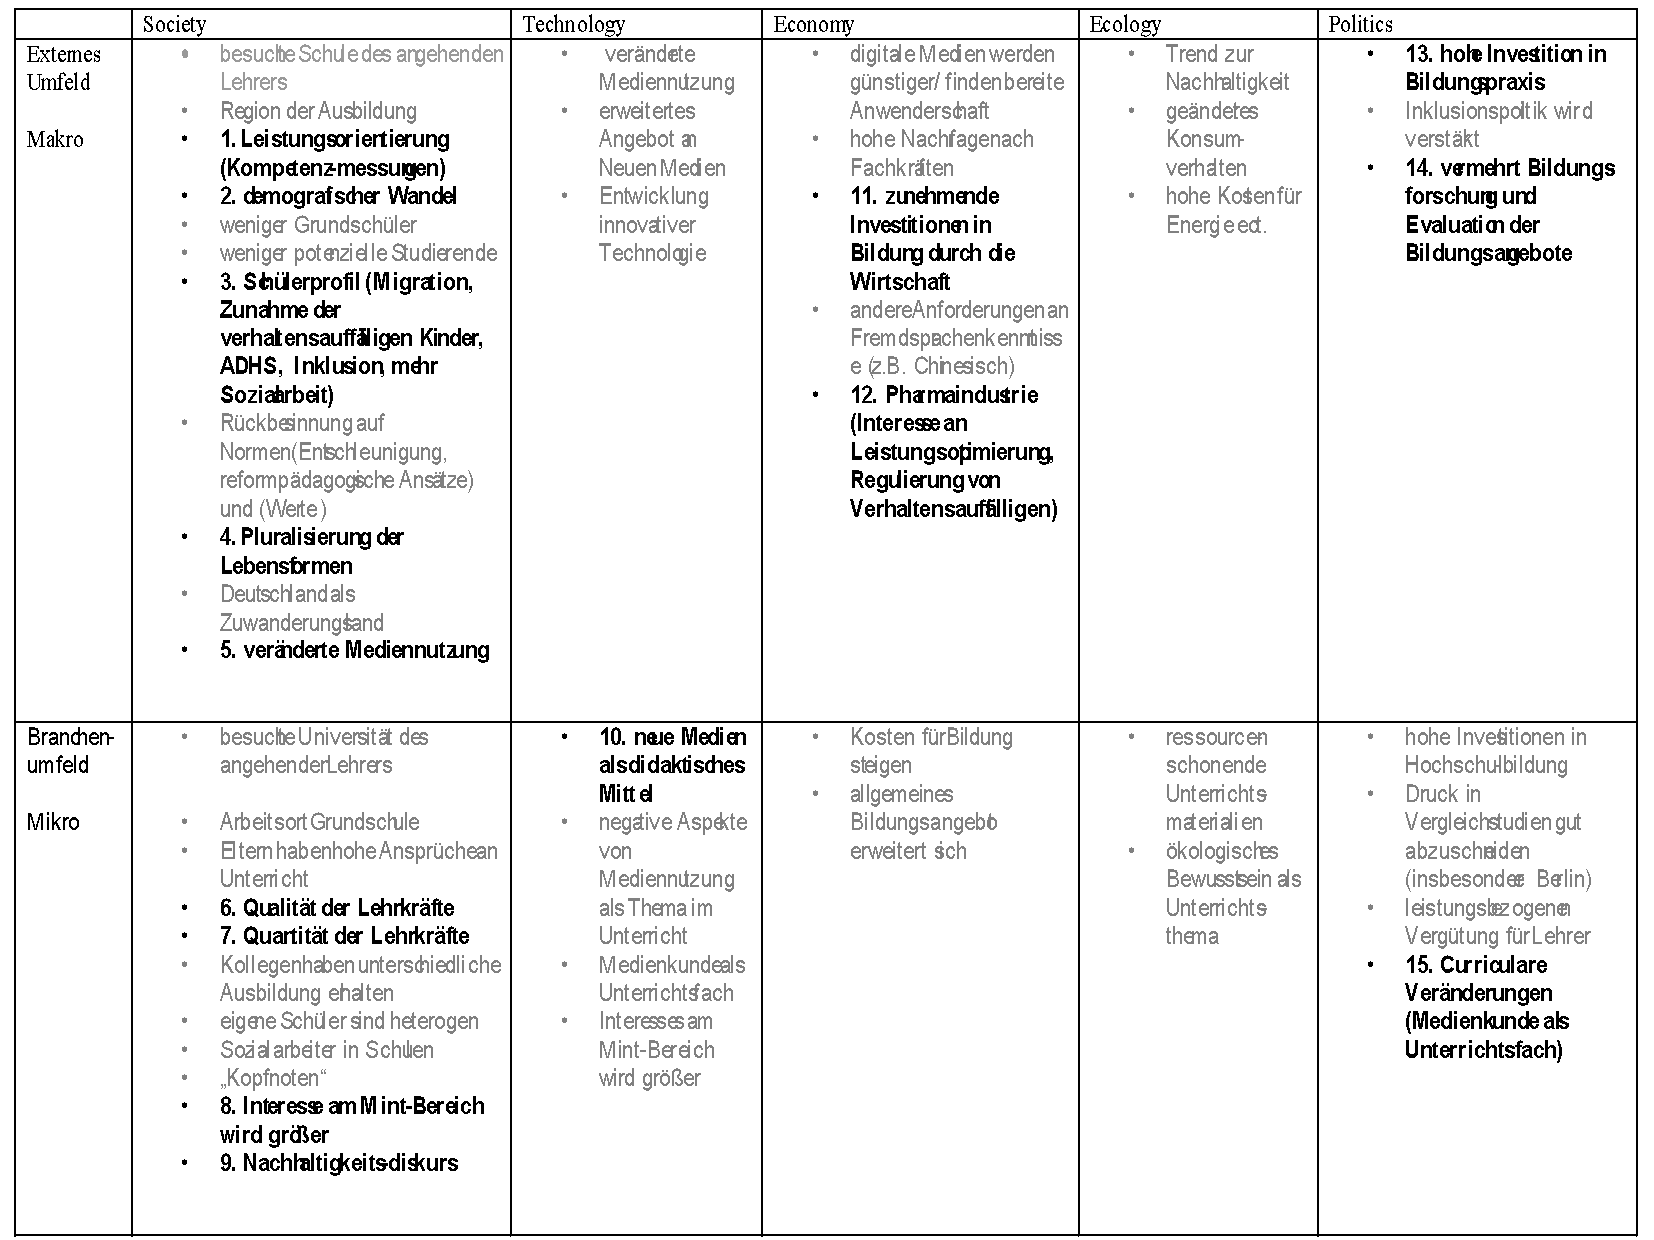
\includegraphics[scale=0.72,angle=90]{pic1.pdf}
\caption{STEEP-Raster}
\label{steep}
\end{table}

Tabelle \ref{steep} stellt die Einflussfaktoren dar, die die Lehrerausbildung im Jahr 2030 beeinflussen können.

\section{Darstellung der Unsicherheitsanalyse Papiercomputer}
\begin{table}[!ht]
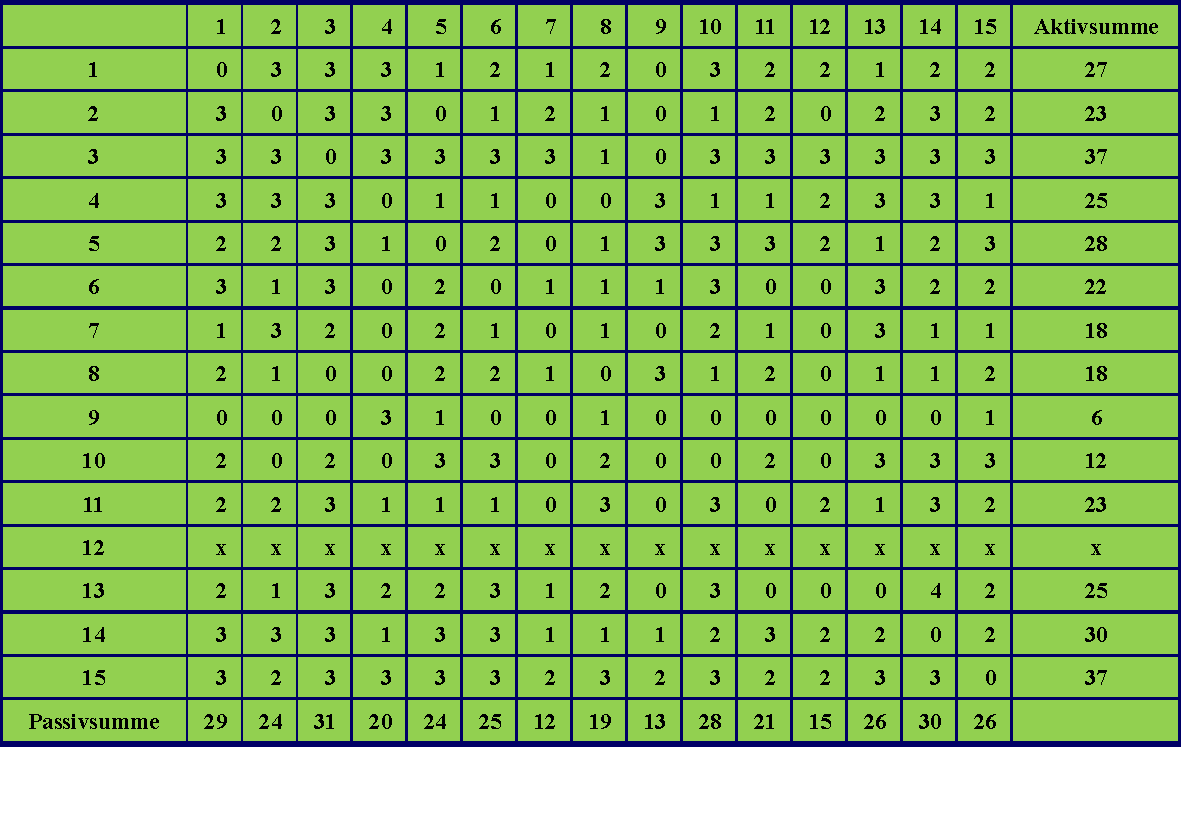
\includegraphics[scale=1.0,angle=90]{tabelle.pdf}
\caption{Papiercomputer}
\label{tabelle}
\end{table}

\section{Darstellung der Unsicherheitsanalyse Papiercomputer}
\begin{figure}[!ht]
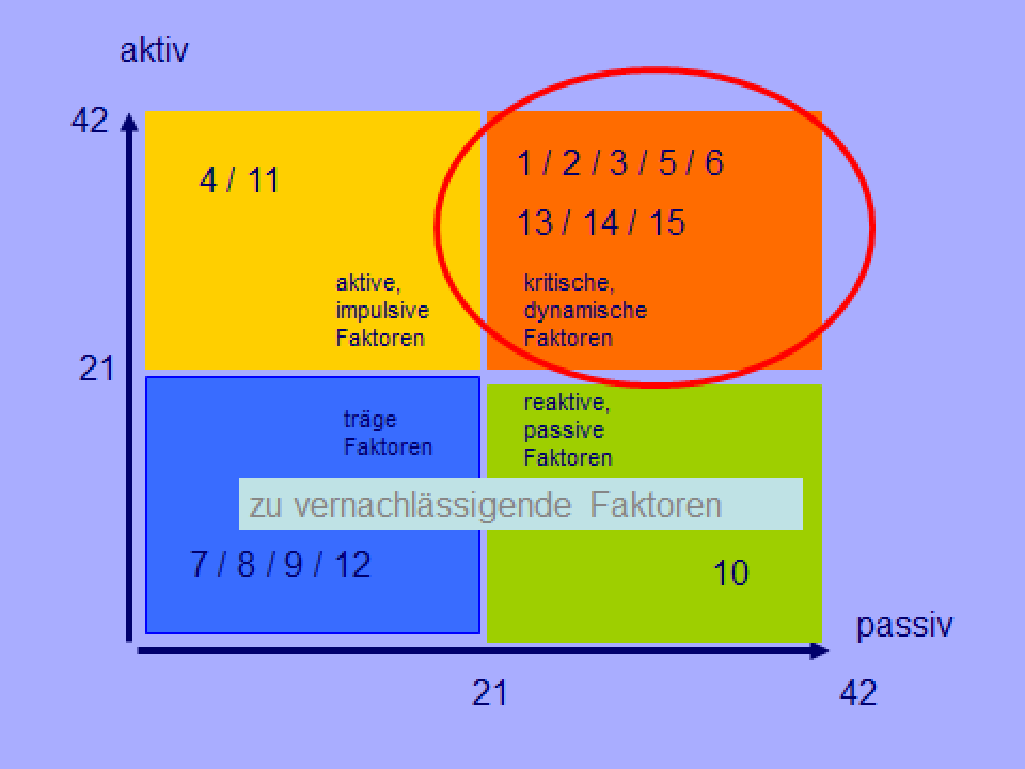
\includegraphics[scale=1.1,angle=90]{faktoren.pdf}
\caption{Faktoren}
\label{faktoren}
\end{figure}

Es konnten acht Schlüsselfaktoren ausgemacht werden, die die Zukunft der Lehrerausbildung beeinflussen können: (1) Leistungsorientierung, (2) demografischer Wandel, (3) Schülerprofil, (5) veränderte Mediennutzung, (6) Qualität der Lehrkräfte, (13) Investition in Bildungspraxis, (14) Forschung und Evaluation der Bildungsangebote, (15) Curriculare Veränderungen.

\section{Darstellung der Projektionen der Schlüs"-sel"-fak"-toren} 
\begin{table}[!ht]
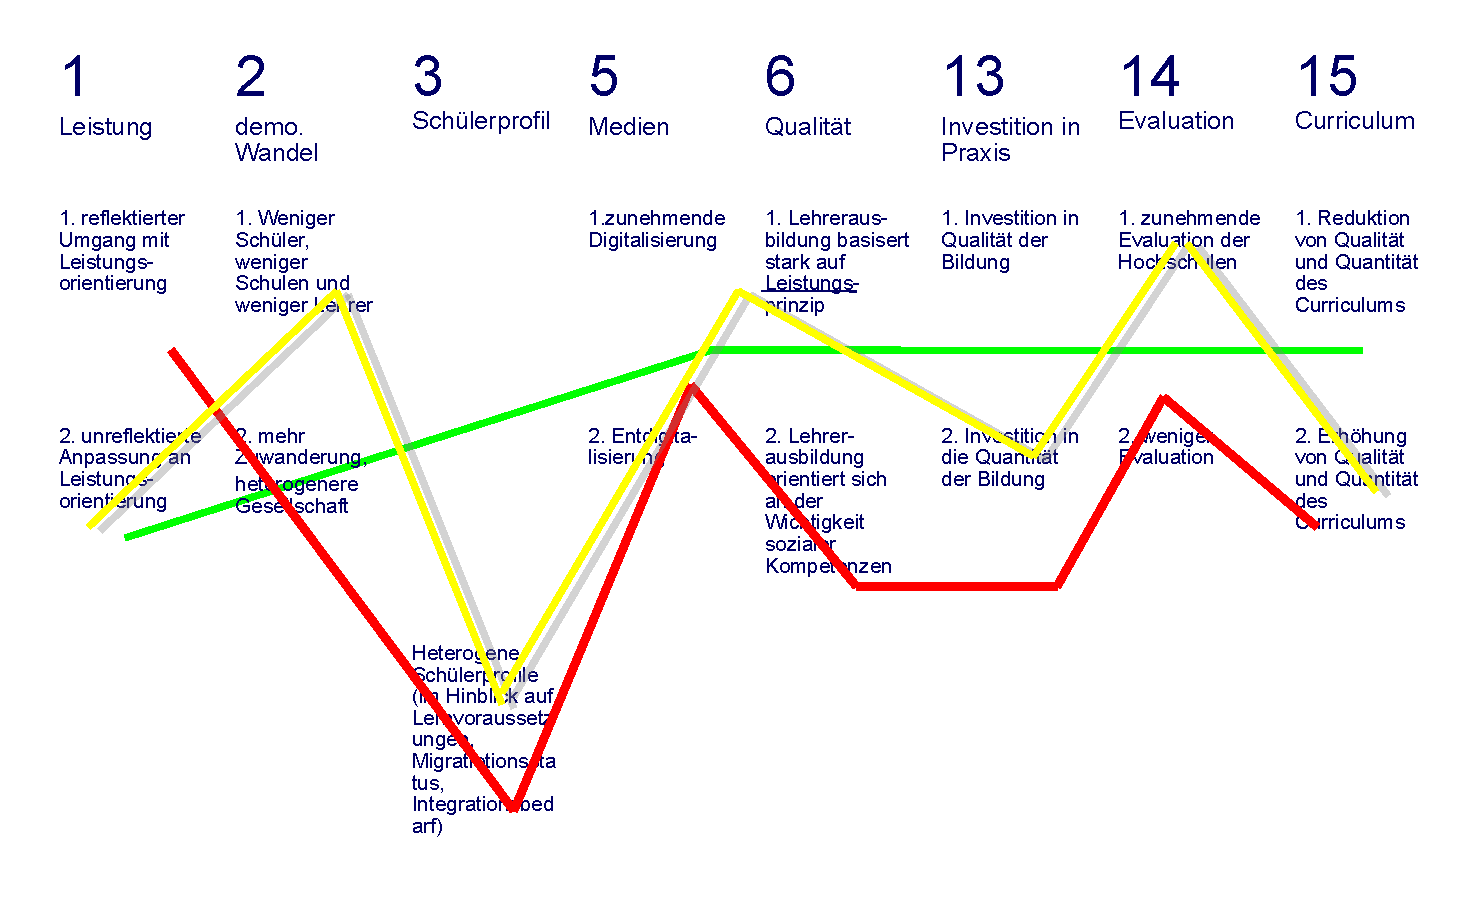
\includegraphics[scale=0.8,angle=90]{projektionen.pdf}
\caption{Darstellung der Projektionen der Schlüsselfaktoren}
\label{projektionen}
\end{table}
In der folgenden Tabelle werden die Projektionen der Schlüsselfaktoren, die von uns formuliert wurden und für den Szenarioprozess relevant sind, aufgezeigt. Aufgrund der entstandenen Projektionen werden die in unserem Fall drei Szenarios ausformuliert. Die farbigen Linien zeigen, dass es drei Szenarios gibt und welche Projektionen bei der Szenarioentwicklung einbezogen wurden. Der rote Pfad: Szenario „Individualisierung und Digitalisierung“, der grüne Pfad: Szenario „Homeschooling“ und der gelbe Pfad Szenario „Leistungsorientierte Gesellschaft“.


\section{Darstellung der Konsistenzmatrix}
Die Konsistenzanalyse dient dazu „den Möglichkeitsraum über unterschiedliche denkbare Ausprägungen aller Schlüsselfaktoren aufzuspannen“ (vgl. Kosow/Gaßner 2008, S. 41)\cite{Kosow2008}. Somit wird deutlich welche Kombinationen von Projektionen sich konsistent zu einander verhalten und auf diese Weise für die Konstruktion konsistenter Szenarien geeignet sind. Die Konsistenz ist entscheidend für die Glaubwürdigkeit der Szenarien. Ziel ist es die Zukunftsprojektionen auf Widerspruchsfreiheit zu überprüfen. Zunächst werden die Ausprägungsmöglichkeiten aller Schlüsselfaktoren in einer Konsistenzmatrix schematisch festgehalten. Danach wird jede Ausprägung mit allen anderen Ausprägung kombiniert und bewertet. Das heißt, dass die Konsistenz der Kombination beurteilt wird. Zur Beurteilung dient ein 5-skaliges Bewertungsschema: 1 = totale Inkonsistenz, 2 = partielle Inkonsistenz, 3 = neutral oder voneinander unabhängig, 4 = gegenseitiges begünstigen sowie 5 = starke gegenseitige Unterstützung (vgl. Kosow/Gaßner 2008, S. 41-42). 

weil das manchmal auch ohne funktioniert und man sich den pfad auch logisch erklaeren kann ohne ne analyse 


\section{Fazit}
In einem Szenario-Prozess der von Studierenden seminarbegleitend durchgeführt wird, sollte beachtet werden, die Faktoren so weit wie möglich einzugrenzen und die Bedeutung der Einflussfaktoren herauszufiltern. Außerdem sollten Zusammenhänge genau betrachtet werden, sonst könnten zu viele Verknüpfungen entstehen, die es schwierig machen sich auf wenige Szenarios zu beschränken. Denn zu viele Einflussfaktoren sprengen den zeitlichen Rahmen, um die Szenarien ausführlich auszuarbeiten. 
Die Szenario-Methode hat sich in Anbetracht der Ergebnisvielfalt gelohnt. Es können Entwicklungen sichtbar gemacht werden, die möglicherweise unter anderen Umständen nicht beachtet werden würden, und somit negative Auswirkungen mit sich bringen könnten. 
Als wichtige und unabdingbare Ressourcen für die Arbeit mit der Szenario-Methode sehe ich zum einen Zeit und zum anderen Kreativität. Zeit benötigt man um Ideen zu entwickeln und die Kreativität spielt für die Projektionenbildung und deren Ausdehnung in alle Richtungen eine wichtige Rolle. Darüber hinaus ist es sinnvoll, dass die einzelnen Prozessschritte eingehalten werden. Die einzelnen Arbeitsschritte schaffen Transparenz und Reliabilität. Eine bestimmte Methodenvielfalt ist angebracht, wenn man feststellt, dass ein „Werkzeug“ nicht greift. 
Ein wichtiges Kriterium für eine erfolgreiche Anwendung der Szenario-Methode ist letztlich die Zusammenstellung der Arbeitsgruppe, die Motivation und die Art der Zusammenarbeit. Die Arbeitsgruppe ist der Ort für ständige Rückkopplung und Austausch von Ideen, Hintergrundwissen und Methoden.

\pagebreak

\bibliographystyle{alphadin} 
\bibliography{Forschungsprotokoll}

%Literaturverzeichnis
%
%Entschließung des 206. Plenums am 21.2.2006. Empfehlung zur Zukunft der Lehrerbildung in den Hochschulen. HRK Hochschulrektorenkonferenz.
%Die Stimme der Hochschulen
%
%Kosow, H.; Gaßner, R.: Methoden der Zukunfts- und Szenarioanalyse - Überblick, Bewertung und Auswahlkriterien. Institut für Zukunftsstudien und Technologiebewertung, Berlin 2008.
%
%Kreibich, R.: Zukunftsfragen und Zukunftswissenschaft. Institut für Zukunftsstudien und Technologiebewertung, Berlin 2006. 
%
%von Reibnitz, U.: Szenario-Technik - Instrumente für die unternehmerische und persönliche Erfolgsplanung. Wiesbaden 1992. 
%
% Albers, O.; Broux, A. (1999). Zukunftswerkstatt und Szenario-Technik. Ein Methodenbuch für Schule und Hochschule. Beltz
%
%Schaefers, Christine
%Forschung zur Lehrerausbildung in Deutschland – eine bilanzierende Übersicht
%der neueren empirischen Studien Schweizerische Zeitschrift für Bildungswissenschaften 24 (2002) 1, S. 65-90
%
%Digitale Medien als Mittel und Inhalt der Lehrerinnen- und Lehrerbildung –
%Medienpädagogische Grundlagen und Beispiele
%Gerhard Tulodziecki, Universität Paderborn, Fakultät für Kulturwissenschaften
%Vortrag im Rahmen der Impulstagung an der PHZ Schwyz: ICT in der Lehrerinnen- und
%Lehrerbildung, 14.05.04
%
%%Ein Bericht von der didakta 2007 in Köln und mehr. (Medien in der Schule – Fehlanzeige?). 2007, Heft 2. 
%%Studie Bildung 2.0 - Digitale Medien in Schulen, BITKOM -Bundesverband Informationswirtschaft, Telekommunikation und neue Medien e.V. 2010). \url{http://www.bitkom.org/de/themen/54629_66034.aspx}
%
%Middendorf, E. (2002). Computernutzung und Neue Medien im Studium. Ergebnisse der 16. Sozialerhebung des Deutschen Studentenwerkes (DSW). Bonn.
%
%Lewin, Karl; Heublein, Ulrich (1998): Berufliche Orientierung, Zurechtfinden im Studium und Computerkenntnisse von Studienanfängern. Hannover. Verlag: HIS-Hochschul-Informations-System 
%
%Bonfiger, J. (2004). Neue Medien im Fachunterricht: eine empirische Studie über den Einsatz neuer Medien im Fachunterricht an verschiedenen Schularten in Bayern. Donauwörth : Auer.

\pagebreak

\begin{appendix}
\section*{Anhang}
\addcontentsline{toc}{section}{Anhang}
\normalsize
\section{Szenario 1: Home-Schooling an der Berliner Grundschulen}
Emil ist 8 Jahre alt und lebt mit seinen Eltern in Berlin-Grunewald. Sein Vater arbeitet als Rechtsanwalt, die Mutter ist Ärztin. Als Emil im Jahr 2030 geboren wurde, wurde hinsichtlich der Schulpflicht eine gesetzliche Änderung bzw. eine Erweiterung vorgenommen, die Emils Eltern mit Freude erfüllte. „Homeschooling“ wurde zu einer anerkannten Form der Beschulung. Staatliche Lehrpläne und ausgebildete Lehrkräfte sind Bestandteile des „Homeschooling“, welches über sog. „E-Teaching Center“ koordiniert wird. Emils Eltern beschlossen schon im Jahr der Geburt ihres einzigen Sohnes: „Das ist das Beste für unseren Emil“. Besonders die Mutter von Emil war am Homeschooling interessiert. Sie kommt aus den USA und dort wird Homeschooling schon längst praktiziert. Es gab auch andere Gründe, warum sich Emils Eltern für Homeschooling entschieden haben. Als erstes waren sie vom Bildungsniveau, welches traditionelle Schulen anbieten, nicht ganz überzeugt. Sechs Wochen nach der Einschulung fragte Emil eines Tages seine Eltern: „Wann werde ich endlich etwas lernen?“ Zweitens war Emil schon in den ersten Wochen seiner Schulzeit leider von Mobbing betroffen. Seine Eltern mussten schnell handeln, so konnte es nicht weiter gehen. Jetzt, nachdem sie sich für Homeschooling entschieden haben, brauchen sie sich keine Sorgen mehr um Mobbing, Gewalt oder Stress in der Schule sowie um die überfüllten Klassen machen. Weiterhin wollten seine Eltern, dass Emil intensiver in bestimmten Bereichen gefördert wird, wie z.B. im Bereich Naturwissenschaften. Dabei sollten auch die geisteswissenschaftlichen Fächer nicht vernachlässigt werden. Der wichtigste Grund für Homeschooling dennoch war, dass er mehr Freiheit, Flexibilität und Wahl im Bildungsprozess anbot als die traditionellen Schulen. Emil kann seinen Stundenplan selbständig erstellen. Wenn er diese Woche Mathematikunterricht den anderen Fächern vorzieht, ist es überhaupt kein Problem. Die Selbstbestimmung, Eigenständigkeit und das Gefühl für Freiheit und Demokratie ist ein Bestandteil des Homeschooling.
Jetzt, acht Jahre später, zahlen die Eltern von Emil monatlich 1.500 Euro für diese in hohem Maße individuelle Bildung ihres Sohnes. Der Lehrplan wurde individuell an Emils Entwicklungsniveau angepasst. An der Erstellung des Lehrplanes waren Emil und seine Eltern aktiv beteiligt. Jeder Wunsch und Hinweis von der Beteiligten wurde berücksichtigt. Homeschooling erlaubte Emils Eltern, ein ganz individuelles Curriculum für Ihren Sohn zu erarbeiten. Dadurch dass der E-Learning-Unterricht individuell an jedes Kind angepasst ist und sich auf das individuelle Lerntempo jedes Kindes orientiert, braucht Emil keine Nachhilfe mehr. Aus diesem Grund eignet sich diese Lern- und Lehrform besonders gut auch für die zugewanderten Kinder, die z.B. anfangs vielleicht mehr in der entsprechenden Sprache gefördert werden sollen und erst später mit anderen Fächern beginnen können.
Emil bekommt keine Zensuren, weil diese als Bewertungs-, Druck- und Selektionsmittel gelten. Auch auf die Tests und Prüfungen wird verzichtet, damit kein Leistungsdruck und keine Vergleiche bei Kindern aufgrund der Noten entstehen. Die Tests werden nur geschrieben, um zu schauen, auf welchem Entwicklungsstand sich die Kinder zu bestimmten Zeitpunkten befinden. Die Leistungsorientierung basiert sich nicht auf der Konkurrenz, sondern vorrangig auf der Motivation und Freude am Lernen jedes einzelnen Kindes. Die Lernbegleiterin von Emil Frau Schmidt fertigt jede 3 Monate ein Portfolio über den Entwicklungsstand seiner Leistungen an. Wenn Emil sich in dieser Zeit besonders viel Mühe gegeben hat, bereitet Frau Schmidt für ihn eine Überraschung vor.
Gewöhnlich beginnt die Woche in der Familie Ehrling so: Emil sitzt in der Küche und frühstückt. Patricia, das mexikanische Kindermädchen ermahnt ihn: „Emil, iss und träume nicht vor dich hin. Es ist gleich 7.45 Uhr. Du musst noch Zähne putzen und dich um 8.00 Uhr im „Teaching-Center“ einloggen. Frau Schmidt wartet nicht auf dich.“
Frau Schmidt hat in ihrer Lehrerausbildung eine Zusatzqualifikation für E-Teaching gestütztes Homeschooling  absolviert. Der Schwerpunkt ist das frühzeitige Heranführen an einen sicheren Umgang mit der Medien-, Informations- und Wissensgesellschaft über die Initiierung weitgehend selbstgesteuerter Lernprozesse.
Um Punkt 8.00 Uhr ist Emil mit seinem Headset ausgerüstet und sitzt in seinem Arbeitszimmer vor dem Rechner. Die erste Schulstunde kann beginnen. Frau Schmidt begrüßt ihn und sogleich beginnt der Deutschunterricht. Das läuft folgendermaßen ab: Emil erhält Anweisungen und Hinweise, was und in welcher Form er in den nächsten 40 Minuten erledigen soll. Nach 40 Minuten treten die beiden wieder in Kontakt und besprechen die Ergebnisse. Anschließend hat er noch Spanisch mit Frau Gonzalez, danach 90 Minuten Mathematik. Zum Mittag loggt er sich aus. Emil ist an eine bestimmte Zeit gebunden, die er in der Woche abarbeiten muss.
Am Nachmittag muss er Hausarbeiten machen, natürlich alles online. So geht das bis Donnerstag. Nur am Freitag findet kein „Homeschooling“ statt. Freitags treffen sich alle Homies im „E- Teaching Center“ und erstellen gemeinsam mit den LernbegleiterInnen eine Wochenbilanz, bevor die Aktivitäten absolviert werden, die physische Anwesenheit erfordern. Das „Science and Universe Center“ und die Experimentierküche „Junge Forscher“ befinden sich im E-Teaching Center“, ebenso die Turnhalle. Emil freut sich immer auf den Freitag, denn es ist der einzige Tag in der Woche, an dem er seine Schulfreunde sieht. Dennoch stehen alle täglich über schoolskype eifrig miteinander in Kontakt. Schüler aus den staatlichen Schulen kennt er eigentlich nicht. Er hat ja auch so genug Freunde…in seinem Freizeitaccount „Friendbook“ sind es 250 Personen, die  aus der ganzen Welt kommen. Es gibt dort viel zu bereden und man kann sich jederzeit auf den neuesten Stand bringen, was gerade „technisch“ aktuell ist.
Auf die nächste Woche freut sich Emil besonders. Frau Schmidt hat ihm erzählt, dass ab nächster Woche in Berlin Evaluation von Homeschooling stattfindet. Homeschooling hat mittlerweile ein großes Interesse in der Gesellschaft geweckt. Da es verschiedene Homeschooling Anbieter gibt, ist Evaluation notwendig geworden. Insbesondere Eltern sind an den Evaluationsergebnissen interessiert.
Aber Emils Mutter interessieren die Ergebnisse der Evaluation nicht so sehr, sie ist in letzter Zeit etwas um ihren Sohn besorgt. Sie ist ja beruflich stark eingebunden, deshalb hat sie sich geärgert, dass Patricia ein paar Tage gewartet hat, bis sie ihr erzählt hat, dass der Emil jetzt wieder häufiger über Bauch- und Kopfschmerzen klagt. Und die Neurodermitis ist auch wieder schlimmer geworden. Na zum Glück ist Emils Mutter Ärztin.
Aber dass er jetzt auch noch Papas geliebte Guppys vergiftet hat, geht entschieden zu weit. Von wegen „ich wollte nur ein Experiment machen“. Emils Mutter versteht das nicht. Der Junge hat doch alles. Sie muss jetzt handeln und vereinbart über Skype mit einem befreundeten Kinderpsychologen einen Onlinetermin für Emil.

\section{Szenario 2: Individualisierung \& Digitalisierung}
Julia ist Studentin im letzten Jahr ihres 5-jährigen Grundschullehrerstudiums. Sie kam mit 19 Jahren nach Deutschland, direkt nach dem Abitur. Zunächst war sie Au-Pair bei einer deutschen Familie. Sie lernte dort sehr schnell deutsch, sodass sie nun 3 Sprachen fließend spricht. Sie interessiert sich für ein pädagogisches Studium und verfolgt daher die jährlich veröffentlichten externen Evaluationsberichte der Hochschulen in Deutschland, sehr aufmerksam. Die FU gilt hierbei als die beste Universität, die Praxis und die Forschung betreffend. Bildungswissenschaftlerinnen der FU waren es, die die Schulstukturreform in Zusammenarbeit mit der Politik maßgeblich vorangetrieben haben. Da in vielen Studien der frühe Übergang in weiterführende Schulen eng mit der Frage sozialer Ungleichheit verbunden ist, wurde in einem zähen Umstrukturierungsprozess, das Schulsystem umgestellt, angelehnt an die finnische Grundschule. Diese umfasst nun 6 Jahre, daran schließt sich ein dreijähriger Oberunterricht an, nach dessen Absolvierung die offizielle Schulpflicht beendet ist und bei Bedarf zwischen gymnasialer Oberstufe und Berufsschule gewählt werden kann. Alle Schulen sind als Ganztagsschule organisiert und eng mit außerschulischen Bildungseinrichtungen wie Sprachschulen in Kontakt.
Julias Mehrsprachigkeit sowie ihre bereits vorhandene pädagogische Kompetenz bildeten einen Vorteil bei einem Auswahlgespräch und dem Motivationsschreiben für die Aufnahme eines Studiums, da händeringend nach mehrsprachigem Lehrkräften gesucht wird, die in multinationalen Klassen unterrichten können. Nicht jeder schafft dieses Auswahlverfahren, zu dem auch noch ein Assessment-Test gehört, in dem psychologische Tests zur Persönlichkeitstestung und Stresstests durchgeführt werden. Dieses Verfahren wurde aufgrund der bisherigen Vergangenheit eingeführt, bedingt durch die Pisa-Schocks und die daraus resultierende Qualitätsdebatte um die Qualität der Lehrerausbildung.
Einmal das Auswahlverfahren geschafft, kann sich Julia über ein hochqualitatives und modernes Studium freuen.
Studieninhalte werden in blended learning Szenarien vermittelt, einer Kombination von virtuellen und nicht-virtuellen Lernsettings und Methoden. Der Gebrauch von Tablets und e-books ist schon längst Alltag und wird finanziell vom Senat und der Wirtschaft gefördert.
Durch die zunehmende Heterogenität in den Klassenzimmern, ist ein Umdenken in den pädagogischen Ansätzen erforderlich. Heterogenität wird nicht mehr ignoriert und als Belastung empfunden, sondern als Bereicherung. Methodisch-didaktisch können dem vor allem adaptive Unterrichtsformen gerecht werden, die die individuellen Voraussetzungen der Schüler fokussieren und den Unterricht an ihre Bedürfnisse anpassen und nicht umgekehrt.
Eine weitere Veränderung ist ein stärkerer Praxisbezug in der Ausbildung. Einmal wöchentlich geht Julia in eine Grundschule, die ihr als Praktikumsstelle von der Uni vermittelt wurde. Hier kann sie, nach der Absolvierung zahlreicher Hospitationsstunden, eigenständig in einem Lehrerteam tätig sein und sich dies auf die spätere Referendariatszeit anrechnen lassen.
Heute ist sie spät dran, schnell checkt sie von unterwegs auf ihrem, von der Schule gestellten, Tablet die Anwesenheit der Klasse, 15 der 25 Schüler haben sich bereits mit ihren Tablets angemeldet, die sie bereits ab der ersten Klasse nutzen.
In der Schule angekommen, trifft sie im Lehrerzimmer auf Herrn Y, einen  aus China stammenden Rentner, der vor über 40 Jahren nach Deutschland kam und bis vor Kurzem als Informatiker tätig war. Er hat einen mehrwöchigen Kurs besucht, der ihn zum pädagogischen Assistenten zertifizierte. Viele ältere Menschen unterstützen ehrenamtlich vor allem den pädagogischen Bereich, sodass der Personalschlüssel verbessert werden kann.
Heute steht das Fach „Medienpädagogik“ auf dem Stundenplan. Seit einigen Jahren ist dies fester Bestandteil des Berliner Curriculums. Es beinhaltet sowohl die Medienerziehung, als auch die Vermittlung praktischen Fähigkeiten, um die Kinder auf die digitalisierte Informationsgesellschaft vorzubereiten. Medienpädagogik kann im Studium als ganz reguläre Fächerkombination gewählt werden, zum Bsp. mit dem Fach Chinesisch, Interkulturelle Kompetenz, Mathe oder Musik.
Doch auch für Julias Kommilitonen mit anderen Fächern, ist Medienpädagogik elementarer Bestandteil des Studiums.
Julias Klasse ist mit 25 Schülern recht groß. In Berlin ist dies jedoch die Regel, trotz des natürlichen Rückgangs der Geburtenzahlen, da Berlin als Zuwanderungsstadt sehr attraktiv ist. Unter den 25 Schülern sind 3 Kinder mit Integrationsbedarf und 12 Kinder, dessen Erstsprache nicht Deutsch ist. Dank verschiedener elektronischer Steuerungs- und Kommunikationshilfsmittel und durch den Einsatz eines Lehrerteams, bestehend aus Klassenlehrer, Speziallehrer und gegebenenfalls eines Lehramtsstudenten, können alle Kinder gleichermaßen in den Unterricht miteinbezogen werden.
Im Studium lernte Julia u. a. den Einsatz sogenannter WebQuests im Unterricht. Dabei handelt es sich um ein computergestütztes Lernarrangement, mit dem die Lernenden sich (meist in Gruppenarbeit) selbständig einen Themenbereich aneignen sollen. Meist handelt es sich um strukturierte Recherche-Projekte zu spezifischen Themen im Internet. Diese können in nahezu allen Fächern eingebaut werden. Die Bearbeitung erfolgt in Kleingruppen, bei deren Einteilung die Lehrerin darauf achtet, die Gruppen möglichst heterogen zusammenzusetzen, so wie sie es in den Vorlesungen zu Lehr-Lern-Prozessen gelernt hat.
Während die Schüler die Aufgaben bearbeiten, geht das Lehrerteam zu den einzelnen Lerngruppen und unterstützt und moderiert die Lernprozesse, durch diskursive Unterrichtsgespräche.
Die Ergebnisse der Arbeitsgruppen werden in der Grundschule nicht mit Noten bewertet, stattdessen erstellen die Lehrerteams in regelmäßigen Abständen Lernbiografien, in denen der Lernstand wertschätzend erfasst wird. Dieser Paradigmenwechsel erfolgte, nachdem erkannt wurde, dass die zu starke Orientierung auf Leistung sich auf die Dauer negativ auf Motivation und Leistung auswirkt. Zwar spielt er auch weiterhin eine zentrale Rolle, jedoch wird er reflektiert betrachtet. Geeignete Bewältigungskompetenzen, um sich dem immanenten Leistungsdruck zur Wehr zu setzen, sind die bereits genannte die Abkehr vom Benotungssystem in der Grundschule und auch die Elternarbeit.
Julia fühlt sich in ihrem Beruf wohl. Sie wird von der Gesellschaft geachtet und unterstützt. Die Erzählungen ihrer Schwiegermutter, selbst seit 30 Jahren im Schuldienst, klingen für sie wie aus einer anderen Welt.

\section{Szenario 3: Lisa - Lehramtsstudentin 2030}
Freitagmorgen der Wecker klingelt: es ist noch früh und sie wird kaum wach das Schlafmittel wirkt noch und so greift sie verschlafen auf den Nachttisch und sucht nach den Aufputschpillen. Sie hat vielleicht 4 Stunden geschlafen nach dem sie gestern nach der Uni noch gearbeitet hat und anschließend noch für die Uni gelernt hat konnte sie trotzdem nicht schlafen, da ihr zu viele Sorgen und Zweifel im Kopf herum schwirrten. Nun ging sie zum Laptop und machte ihn an. Innerhalb kürzester Zeit ertönte eine Stimme die sagte sie haben 10 neue Nachrichten bitte sehen Sie möglichst schnell nach es könnte wichtig sein.  10 neue Nachrichten, dabei hatte sie doch erst vor fünf Stunden nachgesehen.  Von dem Druck geleitet das sie etwas Wichtiges verpassen könnte öffnete sie ihr Emailfach. Eine Mail von ihren Arbeitgeber, der sie bat früher zu arbeiten heute.  Sie arbeitete in der Schule wie alle ihre Kommilitonen. Es war Pflicht als Lehramtsstudentin dort zu arbeiten. Sie waren für die Korrekturen der Leistungstest zuständig die fast täglichen den Lernerfolg der Schüler überprüften. Und neun Mails aus der Uni Arbeitsanweisungen der Dozenten, um auf den heutigen Tag hinzuweisen. Und Erinnerungsmails an die Hausaufgaben für heute. Jeden Tag die Selben Mails die einen  an seine Pflichten erinnerten. Als sie gerade ihren Laptop aus gemacht hatte klingelte ihr Handy. Eine Erinnerungsmail an sie selbst damit sie ihre Unterlagen und Hausaufgaben nicht vergaß mitzunehmen. Als sie schließlich das Haus verließ, um zur Uni zu gehen, ging sie ohne Frühstück, weil ihr die Zeit fehlte. Nur mit Kaffee und Koffeinhaltigen Bonbons lief sie los. In der Uni angekommen schloss sie sich den Massen an die hastig über die Flure strömten aus Angst zu spät zum Seminar zu kommen.  Als sie den Gruppenraum betrat waren bereits die meisten Studenten da auch die Dozentin saß schon am Tisch und startete ihre Digitale Präsentation zum Thema „Pisa 2025“. Seit der erneuten Pisa Katastrophe von 2025 wurde der Druck auf die Lehrer und die Schüler immer größer. Es wurde nun mit noch mehr Disziplin und Lernkontrollen versucht die Schülerleistung zu steigern. Sie nahm ihren Laptop aus der Tasche und stellte ihn an wie ihre Kommilitonen.  Kaum hatte sie ihren Laptop hochgefahren, kam eine Meldung herein. Bitte Test öffnen! In diesem Test wurden wie immer die Hausaufgaben abgefragt, deren Testergebnisse  direkt auf den Laptop der Dozentin gesendet wurden.  Sie bearbeitete die Aufgaben zügig, da sie wusste, dass sie nur 10 Minuten Zeit hatte. Nach 10 Minuten schloss sich der Test automatisch. Und sie wartete bis auch alle anderen ihre 10 Minuten hatten. Dann begann die Dozentin mit dem Unterricht. Die Anzahl der Studenten war gering im Seminar oder generell an der Uni, da das Angebot und die Nachfrage auf Grund des Geburtenrückgangs gering ist, aber das war nicht der einzige Grund viele der Kommilitonen haben bereits im ersten Studienjahr wieder aufgehört, weil sie dem Leistungsdruck der Lehrerausbildung und den zukünftigen Anforderung an den Lehrerberuf nicht gewachsen waren. Nach dem Seminar musste sie zur zentralen Hochschulevaluation. Der Monat war rum und alle Studenten mussten ihren Unterricht evaluieren und damit auch jeder teilnahm hatte man eine zentrale Stelle eingerichtet wo jeder registriert war und so konnte sichergestellt werden das auch alle teilnahmen, wer das nicht tat wurde angemahnt.  Nach der Evaluation ging es zum nächsten Seminar ein Seminar über die Erstellung von Leistungskontrollen. Auch hier wird zunächst einen 10 Minuten langer Test geschrieben. Anschließend hatte sie dann ein Seminar über Lehrmethoden zur Motivationssteigerung der Schüler.  Hier gab es keinen Test aber jeder Student musste eine ausgewählte Lehrmethode vorstellen. Nach dem Unterricht hatte sie endlich Zeit etwas zu Essen, aber auch hier drängte die Zeit da sie noch in die Schule musste zum arbeiten.  Hastig aß sie und eilte dann zur Schule. Sie setzte sich in einen Arbeitsraum,  mit etwa 10 andern Studenten und nahm sich einen Stapel Tests und fing an sie zu korrigieren. Sie saß direkt neben dem Arzneischrank in dem die Medikamente für die Schüler gelagert wurden  wie Ritalin. Nach vier Stunden hatte sie etwa 50 Tests durchgesehen und das Ergebnis war wieder einmal erschreckend. Die Hälfte der Schüler hatte weniger als 50% der Aufgaben richtig und nur etwa 2% hatten hervorragende Ergebnisse erzielt. Nun musste sie noch die Medikamentenschachteln auffüllen und in den einzelnen Klassenzimmern verteilen. Müde ging sie nach Hause wissend, dass sie selbst noch lernen musste für ihre eigenen Tests. Morgen war zwar Samstag aber dort hatte sie trotzdem Unterricht. Ein Blockseminar zum Thema: „Leistungsbezogene Unterrichtsgestaltung“.  Dafür musste sie noch einen Text lesen und durcharbeiten um für den morgigen Test vorbereitet zu sein. Als sie zu Hause ankam war sie völlig müde  und hatte fürchterliche Kopfschmerzen, also schluckte sie erst eine Kopfschmerztablette und anschließend eine weitere Aufputschtablette um die Hausaufgaben noch zu schaffen. Als sie endlich fertig war, war sie durch die Tabletten so wach das sie nicht schlafen konnte, da ihr aber nur noch fünf Stunden bis zum Klingeln des Weckers blieben griff sie erneut zum Nachtisch und schlief schließlich ein.  
\end{appendix}
\end{document}